\documentclass{article}
\usepackage{graphicx}
\usepackage{titlesec}
\usepackage{hyperref}
\usepackage{enumitem}
\usepackage{lmodern}
\usepackage{amsmath}
\usepackage{fancyhdr}
\usepackage{textcomp}
\usepackage{lmodern}% http://ctan.org/pkg/lm
\usepackage[table,x11names,svgnames]{xcolor}
\usepackage{soul}
\usepackage{parskip}
\usepackage{multirow}
\usepackage{array}
\usepackage{afterpage}
\usepackage{tabularx}
\usepackage{float}
\usepackage{placeins}
\usepackage{tablefootnote}
\usepackage{microtype}
\usepackage{textcomp}
\usepackage{titlesec}
\usepackage{enumitem}
\usepackage{listings}
\usepackage{subcaption}
\usepackage{verbatim}
\usepackage[htt]{hyphenat}
\usepackage[letterpaper, portrait, margin=1.5in]{geometry}
\counterwithin{table}{section}
\counterwithin{figure}{section}

% Directives
\setlength\extrarowheight{5pt}

\setcounter{secnumdepth}{4}
\titleformat{\paragraph}
{\normalfont\normalsize\bfseries}{\theparagraph}{1em}{}

\begin{document}



\hrulefill \par
{\Large \textbf{Learn to play Go}\par}
{\Large Proposal\par}
\hrulefill \par
\begin{align*}
\mathrm{Albert\ Liu} &&\href{mailto:albertpl@stanford.edu}{albertpl@stanford.edu}\\
\end{align*}

\section{Introduction}
We formulate the game of Go as a reinforcement problem. The state space is all possible placements of the stones on the board and the player (i.e. black or white), which is fully observable as input. The action space is any legal position the player can put a stone to plus a special "pass" action. We aim to learn the optimal policy through reinforcement learning where out system can produce next action by observing the board. Figure \ref{fig:goboard} shows a concrete Go board and white stone $P15$ is the current move. The main challenge is enormous search space, large number of legal move per state ( $\sim 250$ ) and the difficulty to handcraft a heuristic evaluation function for positions and moves. DeepMind team has made tremendous improvements, particularly AlphaGo \cite{silver2016mastering}, AlphaGoZero \cite{silver2017masteringalphagozero} and AlphaZero \cite{silver2017masteringalphazero} with deep reinforcement learning approaches and self-play.

\section{Evaluation}
We follow the standard setup and assign a reward to the player, 0 if it is tie, -1 if player loses, +1 if player wins. And we use Pachi \cite{baudivs2011pachi} as our game engine and adapt a Python wrapper based on OpenAI's Gym \cite{brockman2016openai} previous implementation. The build-in Pachi engine is said to hold KGS 2d rank and is considered as our oracle.

As for our baseline, we train a 4-layer convolutional neural network by supervised learning to emulate the moves made by expert players. The dataset \cite{FoxGoServer} contains $~140K$ game records in SGF format played by professional players.
\begin{figure}[H]
\begin{center}
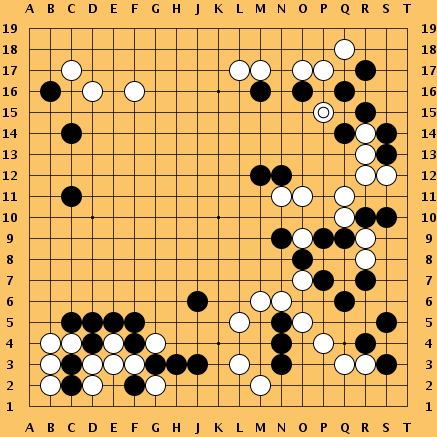
\includegraphics[width=0.5\linewidth]{goboard}
\end{center}
\caption{a snapshot of the Go board}
\label{fig:goboard}
\end{figure}

\bibliography{reference} 
\bibliographystyle{ieeetr}
\end{document}
